\chapter{Analysis}
	
	
	\section{Verification of problem}\label{sec:verification}
		
 	\subsection{Why a problem?}
 	The design process of landscape architects has been more influenced by modern digital technology over the past 50 years, since Harvard's Laboratory of Computer Graphics was established.\cite{landscapeArchitectureDigiTech} In spite of landscape architects being first-movers in exploring digital applications for spatial analysis, many landscape architects are struggling with conceptualizing digital technology as a creative medium\cite{landscapeArchitectureDigiTech}. A survey on members of ASLA (American Society of Landscape Architects)\cite{surveySketchVSDigital}, shows that a 46\% of landscape architects prefer sketching by hand during the design process instead of using digital tools, 31\% prefer using a computer and the remaining 23\% use the computer for efficiency and the hand for creativity. Based on the statements given by the respondents the survey concludes that; \textit{"computers are not intuitive and design is intuitive"}\cite{landscapeArchitectureDigiTech}\cite{surveySketchVSDigital}. Although, computer software enables visualization in 3D which is an effective way of communicating large amounts of complex data to a wide non-expert audience, through visual cues that are more intuitive than those of a 2D-sketch, it can be time-consuming to create 3D visualizations\cite{landscapeVisual}
 	
 	
 	\subsection{Who says so?}
 	
 	\subsection{Why does it matter?}
 	
 	\subsection{Elderly people's approach to technology}
 	Old people typically will not seek out to use state of the art technology, despite its ability to enable experiences that their age would otherwise prevent. As the elderly retire, they have more time on their hands to do whatever they feel like, and for some of these people gardening could be a very possible interest. But often, age lead to a loss of mobility, limiting old people's ability to garden and their enjoyment thereof, leading to a decrease in life quality. Professional teams have created immersive virtual reality applications like AlohaVR \cite{elderlyVRScout} to help people within the elderly age group seize their issues with chronic pain, relaxation, anxiety, and to provide general entertainment.
 	%How does the below sentence relate to the above at all? Surely their lack of mobility has nothing to do with their ability to *design* a garden.
 	So the question could be raised, would it be necessary to have a product that would function for garden designers to work with the elderly and including them in the technological experience? \\
 	
		
		The Pew Research Center has studied the technology adoption of elderly citizens in USA during the last 4 years. They created statistics \cite{seniorTechnology} to show the approach elders to technology as seen in \autoref {fig:oldstats1}. Furthermore the study shows estimates on actual use of different technologies by seniors in the age group 65+ years.
			\begin{figure}[H]
			\centering
			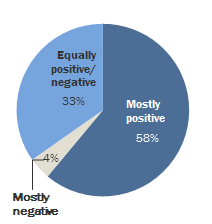
\includegraphics[width=0.4\linewidth]{figure/Analysis/oldpeoplestats1}
			\caption{Elderly peoples approach to technology in society.}
			\label{fig:oldstats1}
			\end{figure} 
		Another statistic shows how large a part of the senior population actually uses Internet and broadband as seen in \autoref{fig:oldstats2}. Nevertheless the graph shows that about 2/3 of the elderly population uses Internet to some extent, which allows the possibility for garden designers to design for the elderly. Furthermore these results creates the chance for garden designers to work with people of all ages, where earlier technology usually would be developed for the use with younger audiences and customers as they were the more common users.
			\begin{figure}[H]
			\centering
			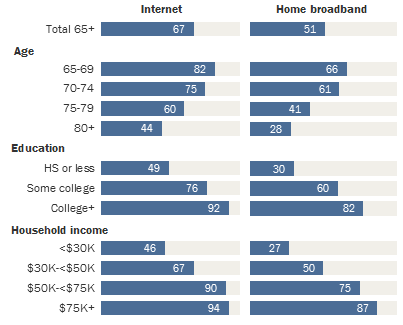
\includegraphics[width=0.6\linewidth]{figure/Analysis/oldpeoplestats2}
			\caption{Elderly peoples use of Internet and Broadband in percent.}
			\label{fig:oldstats2}
		\end{figure} 
		
	\subsection{Interviews}
	
	The target group had been defined as "people who go to gardening centers", and we needed to learn more about this target group. To this end, unstructured interviews were conducted at a garden center with its customers. This way we would get a better understanding of both the target group and the context the product would be used in. We had the option of observing the target group in a natural environment, performing the task that we aim to help them with. Also during this time we had access to staff at the center and could inquire about customer behavior, and any ideas form the staff on our project \\
	% This section is still usable, but should be rephrased to target the garden designers	
	%Also rewrite to reflect that we never met with the employees	
	
	% when and where
	% what does location and time mean for the data
		List of questions for target group
		\begin{itemize}
			\item[-] Have you ever used a garden designer?
			\item[-] What was your experience?
			\item[-] What are you planning to buy?
			\item[-] What are you plan/thoughts for when you buy a new plant?
			\item[-] What do you consider when you buy a new item for your garden?
			\item[-] How often do you make major changes to your garden?
			\item[-] For which reasons did you decide to purchase this item?
			\item[-] What was the latest item you bought that you were not satisfied with?
			\item[-] Do you have a garden?
			\item[-] How did you start the design process?
			\item[-] What tools did you use, if any?
			\item[-] When did you make changes to your garden?
			\item[-] What big changes would you like to make?
			\item[-] Are you retired?
			\item[-] If you had all the time in the world, what would you change about your garden?
			\item[-] Do you enter the garden center with a budget in mind?
			\item[-] Why are you here? \\
		\end{itemize}
		
		List of questions for experts \\
		Target group questions:
		\begin{itemize}
			\item[-] Which people usually addresses you?
			\item[-] What is the most usual demography?
			\item[-] Do people need designing for all or just parts of their garden?
			\item[-] Who makes the 3D visualization of the garden? Is it something you create internally in the company, or does it come from outside cooperators? 
			\item[-] How does this process function?
			\item[-] Do people take the offer on 3D visualization of their garden?
			\item[-] What about development over time? Does it mean that growth can be followed year by year, or does it concern seasons?
			\item[-] Is it something people make use of? \\
		\end{itemize}
		
		Technology questions:
		\begin{itemize}
			\item[-] How do you think a Virtual Reality experience in the 3D environment would be received?
			\item[-] If a customer could design their own garden in a gardening center and instantly visualize it in Virtual Reality, do you think it would be a popular choice? \\
		\end{itemize}
		
		Design questions:
		\begin{itemize}
			\item[-] How large of a garden area do you usually work with?
			\item[-] What plants are trending at the moment?
			\item[-] What is a popular garden style?
		\end{itemize}

		\subsubsection{Demographic information}
		\begin{itemize}
			\item[-] Sex
			\item[-] Age
			\item[-] Job
			\item[-] Marital Status
			\item[-] Level of education
		\end{itemize}
	
	\subsection{Expert Interviews}
		For further validation of the problem 4 phone interviews with landscape architects(Experts) were conducted. 2 of the experts were actively using 3D technology for visualizing garden plans for their customers. The other 2 only used sketching by hand. Due to logistics the interviews were conducted by phone as the experts had their practise at various locations throughout the country. The interviews were semi-structured to allow for new ideas and points to potentially surface. The practical advantages of interviewing over the phone instead of face-to-face interviews were also considered.\cite{telephoneInterview}

	\section{Context}
		
	\section{Target group}\label{sec:targetGroup}
		\subsection{Who are the target }
		
	\section{Technologies}\label{sec:technologies}
		\subsection{Virtual Reality}
			The earliest attempts at a VR experience was in the 1950s\cite{VRS} by Morton Heilig who made the Sensorama\ref{fig:sensorama}; an arcade-style theater cabinet, that featured stereo speakers, stereoscopic 3D display, smell generators, fans and a vibrating chair.
			\begin{figure}[H]
				\centering
				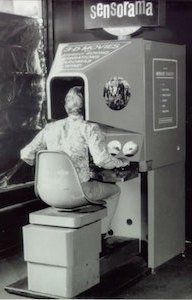
\includegraphics[width=0.4\linewidth]{figure/Analysis/sensorama2}
				\caption{The Sensorama made by Morton Heilig in the 1950s. Fully featured first step at virtual reality.}
				\label{fig:sensorama}
			\end{figure}
			There were a couple of short movies made for the Sensorama, but these were all produced and edited by Morton Heilig himself. The whole setup was stationary, and didn't feature any Head Mounted Display (HMD), so the user had to sit in the vibrating chair and look straight at the display for the duration of the movie. The more modern versions do not include features like smell and fans, but are also geared more towards mobility and full body immersion, and having a vibrating chair doesn't promote that idea.\\
			
			Morton Heilig later went on to further develop the idea of virtual reality, by making the first HMD in form of the Telesphere Mask\cite{VRS} in 1960. This took the immersive nature of his first product to a more personal level, even though it still just were a simple stereoscopic 3D wide view, with stereo sound. It did however look more like the virtual reality headsets of the modern day as seen in \autoref{fig:telesphere}.
			\begin{figure}[H]
				\centering
				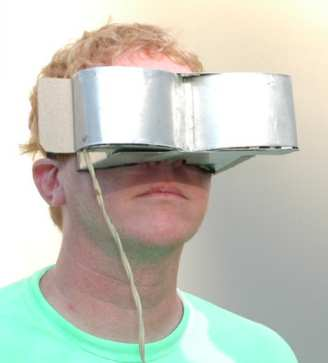
\includegraphics[width=0.25\linewidth]{figure/Analysis/TelesphereMask}
				\caption{The first attempt at HMD virtual reality headset, made by Morton Heilig in 1960. It worked by having stereoscopic 3D vision and stereo sound.}
				\label{fig:telesphere}
			\end{figure}
			Even though it was a step in the direction of a functioning virtual reality headset, it was still only a display showing a movie, it didn't have any motion tracking, or interaction between the user and the movie being watched. There was a sore lack of immersion, which is what makes the virtual reality headsets of today what they are.\\\\

			In 1961 the first motion tracking HMD was developed\cite{VRS}, it was made for military purposes, and was focused on tracking the head movements to control a remote camera. This was to allow a soldier to view remote locations in a natural fashion, without risking the viewer to actually be physically present. It used magnets to accomplish the head motion tracking.\\
			
			After the initial hype for virtual reality died down with the invent of the world wide web in the mid 90's, the industry waited patiently for hardware that could provide the immersion that tied the experience as a whole together. All of the early attempts had one flaw in common; the hardware couldn't provide close to realistic or good looking graphics at a frame rate that wouldn't induce motion sickness in the user, at a price that a normal consumer could afford\cite{vergeVR}. And hence the virtual reality industry laid dormant until 2013 when a certain Palmer Luckey, made a kickstarter for a virtual reality headset called Oculus Rift\cite{createOculus}. This headset kick started (No pun intended) the hype and interest in virtual reality as a medium.
			
			\subsubsection{The essence of VR}
				Virtual reality is a medium\cite{definingVirtualReality}, a medium that has been a long time underway. Starting in the sixties, and being reborn in 2013 by Luckey Palmer, this medium is usually defined by a set of hardware implementations. These hardware implementations range a lot in price and devices, but a broad definition of the medium is:\\

					\begin{quote}
						\textit{Virtual Reality is electronic simulations of environments experienced via head-mounted eye goggles and wired clothing enabling the end user to interact in realistic three-dimensional situations}\cite{coates1992}.\\
					\end{quote}

				This definition is however quite old, being from 1992, but it does still apply to a certain degree to the current state of virtual reality as a device specific medium. Even though the devices, and their capabilities have changed, the way of interaction with the medium is largely the same; Put on a head mounted display, grab the controllers, and explore the 3D world you put yourself into. The rest of the paper will assume the definition of virtual reality as being:\\
				\begin{quote}
					\textit{Virtual Reality is electronic real time simulations of environments experienced via head-mounted eye goggles and one or more controllers enabling the end user to interact in realistic three-dimensional situations}\label{def:virtualRealityDefinition}.\\
				\end{quote}
				 
			\subsection{Fiducial markers}\label{sec:fiducialMarkers}
				By measuring fiducial marker systems, regarding their performance, it is possible to rate the markers by how reliably it finds image points matching physical points on the markers. There can be several reasons to why a fiducial marker system would have problems working or live up to the desired performance. This is typically; poor tolerance to lightning conditions and cluttered scenes causing similar markers to be mistaken by each other\cite{fiducialMarkers}. These problems may complicate the system design.\\
				
				There are however a way to figure out if the fiducial marker system is useful and reliable. This can be characterized by some numerical metrics and some qualitative observations, made with carefulness;\\
				\begin{enumerate}
					\item the false positive rate,
					\item the intermarker confusion rate,
					\item the false negative rate,
					\item the minimal marker size,
					\item the vertex jitter characteristics,
					\item the marker library size,
					\item immunity to lighting conditions,
					\item immunity to occlusion,
					\item perspective support,
					\item immunity to photometric calibration, and
					\item the speed performance.\\
				\end{enumerate}
				
				Failing to properly address these criteria will reduce the usability of a marker system remarkably\cite{fiducialMarkers}. All of the numbers have a valid reason for them to be announced; The false positive rate is falsely reporting the presence of a marker when none is present. The intermarker confusion rate is when one marker is mistaken for another. The false negative rate is when the marker can be seen on an image, but not reported. The minimal marker size is the size of the pixels required for the system to detect the marker. The vertex jitter is the noise in the marker corner positions. The library size is the number of unique markers the system is capable of storing. Two important things from the list is immunity to lightning conditions and immunity to occlusion, for a fiducial marker system it is crucial that the system is able to detect and recognize the markers despite the ambient lighting and partial covering of the pattern.\\
				Last is to mention the practical issue of speed performance. A vision-based fiducial marker tracking system must function in real time, using a low cost computing power, for it to be considered useful.\\
				
				All these criteria can be highly fulfilled using a system called ARTag \cite{fiducialARTag}. ARTag consists of a library of patterns with a square border and unique interior digital signature, along with the possibility to detect algorithms found in imagery \cite{fiducialMarkers}.\\
				
				It is important to state here, that not every kind of pattern in a marker is suitable when it comes to fiducial markers\cite{fiducialMarkers}. As an example it is worth mentioning bar codes as seen in \autoref{fig:fiducialmarkers}, these are not suitable as fiducial markers, because they are made to be read by a laser scanner.\\
				Alongside bar codes follows QR. There are two reasons for this; in fiducial marker systems a large field of view is usually preferred. therefore QR is not suitable for this, mainly because they are not intended for this kind of system.This will cause perspective distortion and they will not provide enough image points for 3D pose calculation.The second reason that QR is not suitable is because they require a large area in the image, this will limit the range as to where the markers can be used.\\ 
				
				
					\begin{figure}[H]
						\centering
						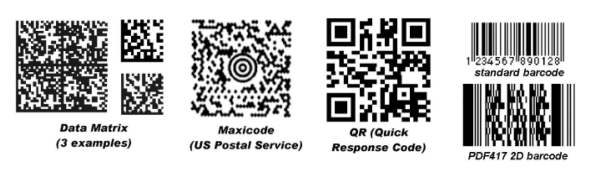
\includegraphics[width=0.9\linewidth]{figure/Analysis/fiducialmarkers.png}
						\caption{Different markers, not suitable for a fiducial marker system.}
						\label{fig:fiducialmarkers}
					\end{figure}
					
				
				As stated above, there are a lot of different markers that can be used for a fiducial marker system, but some are more efficient than others, as seen in \autoref{fig:fiducialworking}, depending on what kind of system will be used.
				Fiducial marker systems is usually functioning in two different stages; hypothesis generation and verification/identification.\\
				
				\begin{figure}[H]
					\centering
					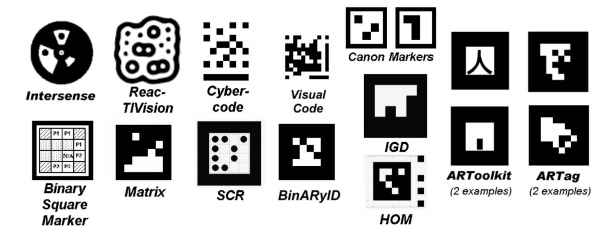
\includegraphics[width=0.9\linewidth]{figure/Analysis/fiducialworking.png}
					\caption{Different markers, suitable for a fiducial marker system.}
					\label{fig:fiducialworking}
				\end{figure}
				
				
		\subsection{Image Processing}
			\subsubsection{Color detection}
			
			\subsubsection{Edge detection}
			
			\subsubsection{Blob detection}
			
			\subsubsection{Object recognition}

    \section{State of the art}\label{sec:SOTA}
		
		\subsection{VR Gardens}
			VR Gardens is a mobile application for designing and planning your own garden. It contains a variety of different 3D models of trees, bushes, outdoor furniture, tiles and the like, to help visualise any garden idea one might have. The design can then be reviewed using the Google Cardboard or similar simple Virtual Reality boxes to be immersed in a close-up edition of the design.
			\begin{figure}[H]
				\centering
				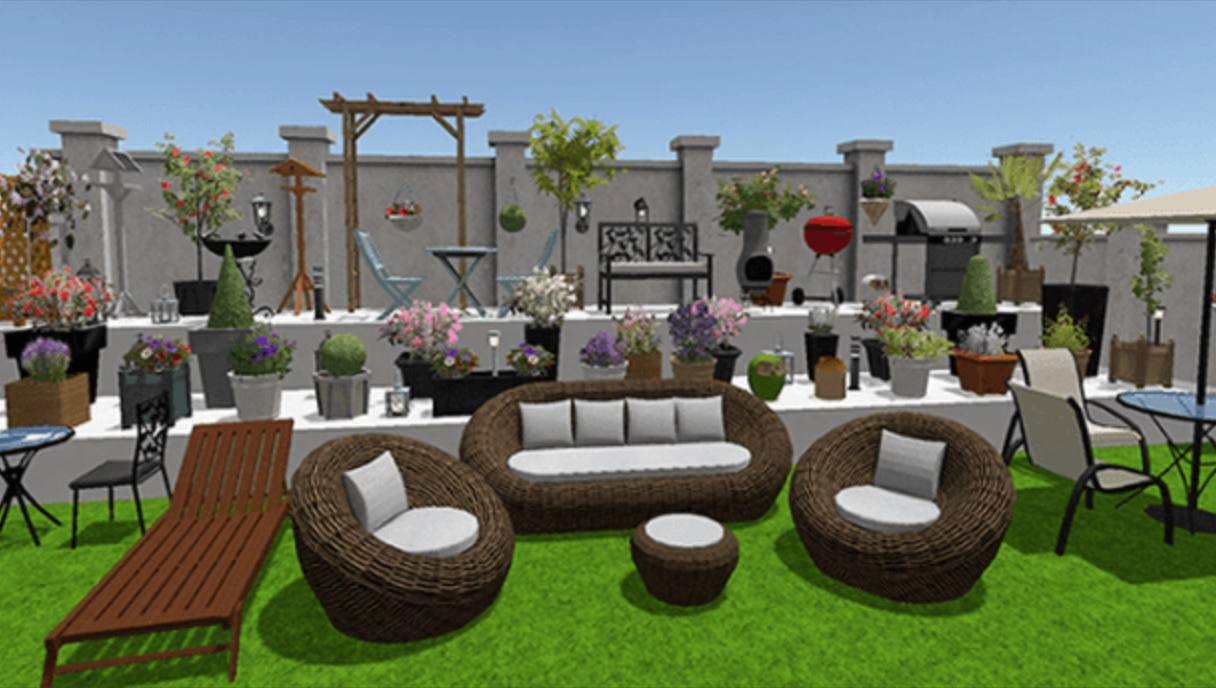
\includegraphics[width=0.6\linewidth]{figure/Analysis/vrgardens}
				\caption{VR Gardens comes with many pre-rendered 3D models}
				\label{fig:vrgardens}
			\end{figure}
			
		\subsection{Mental Canvas}
			A software system that combines 2D draw-and-paint with 3D\footnote{Mental Canvas: \url{https://www.mentalcanvas.com}} which enables a user to create a 3D environment from sketches, supporting conceptual architectural design and analysis. It has been created for Microsoft's Surface technologies\footnote{Microsoft Surface: \url{https://www.microsoft.com/en-us/surface}} and is compatible with the Surface Dial. The system allows for the user to place 2D surfaces, or \textit{canvases} in a 3D space using traditional CAD(Computer-Aided Design) tools of positioning, scaling, rotating on XYZ-coordinate axes.\cite{sotaMentalCanvas}
			
				\begin{figure}[H]
					\centering
					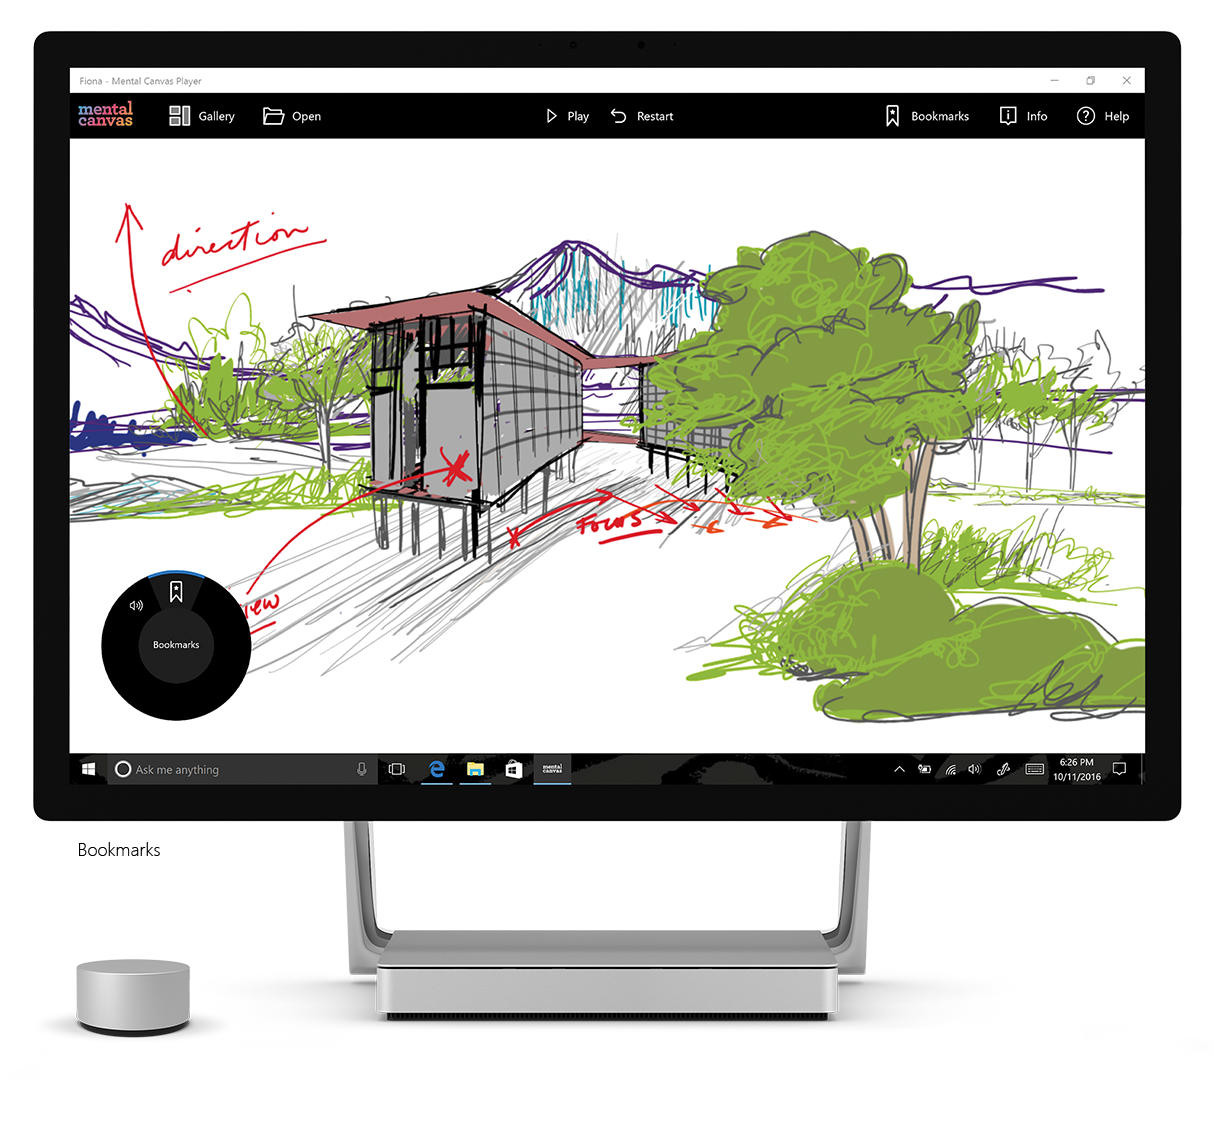
\includegraphics[width=0.5\linewidth]{figure/Analysis/mentalCanvas.png}
					\caption{Mental Canvas combines 2D sketching systems with 3D computer systems.}
					\label{fig:mentalCanvas}
				\end{figure}

		
		\subsection{Reactable}
			reacTIVision\footnote{reacTIVision: \url{http://reacTIVision.sourceforge.net/}} is a framework for developing computervision applications and interfaces. It uses fiducial markers as seen in  \autoref{sec:fiducialMarkers} to sense objects and movement, which allows for more extended interaction. \\
			
			Reactable\footnote{Reactable: \url{http://reactable.com/}} is a musical instrument that uses the reacTIVision framework, to map different controllers on a tabletop interface. The different types of fiducial markers displayed on cubes or small figures work as knobs, buttons and the like to imitate an analog synthesizer, but with different more visual interactions. It enhances the musician's or sound engineer's chance to be more visually creative with their music. The table itself consists of a camera at the bottom pointing upwards to the tabletop. The camera detects interactions made by the user and how the fiducial markers are altered, which results in a musical sound space.
				\begin{figure}[H]
					\centering
					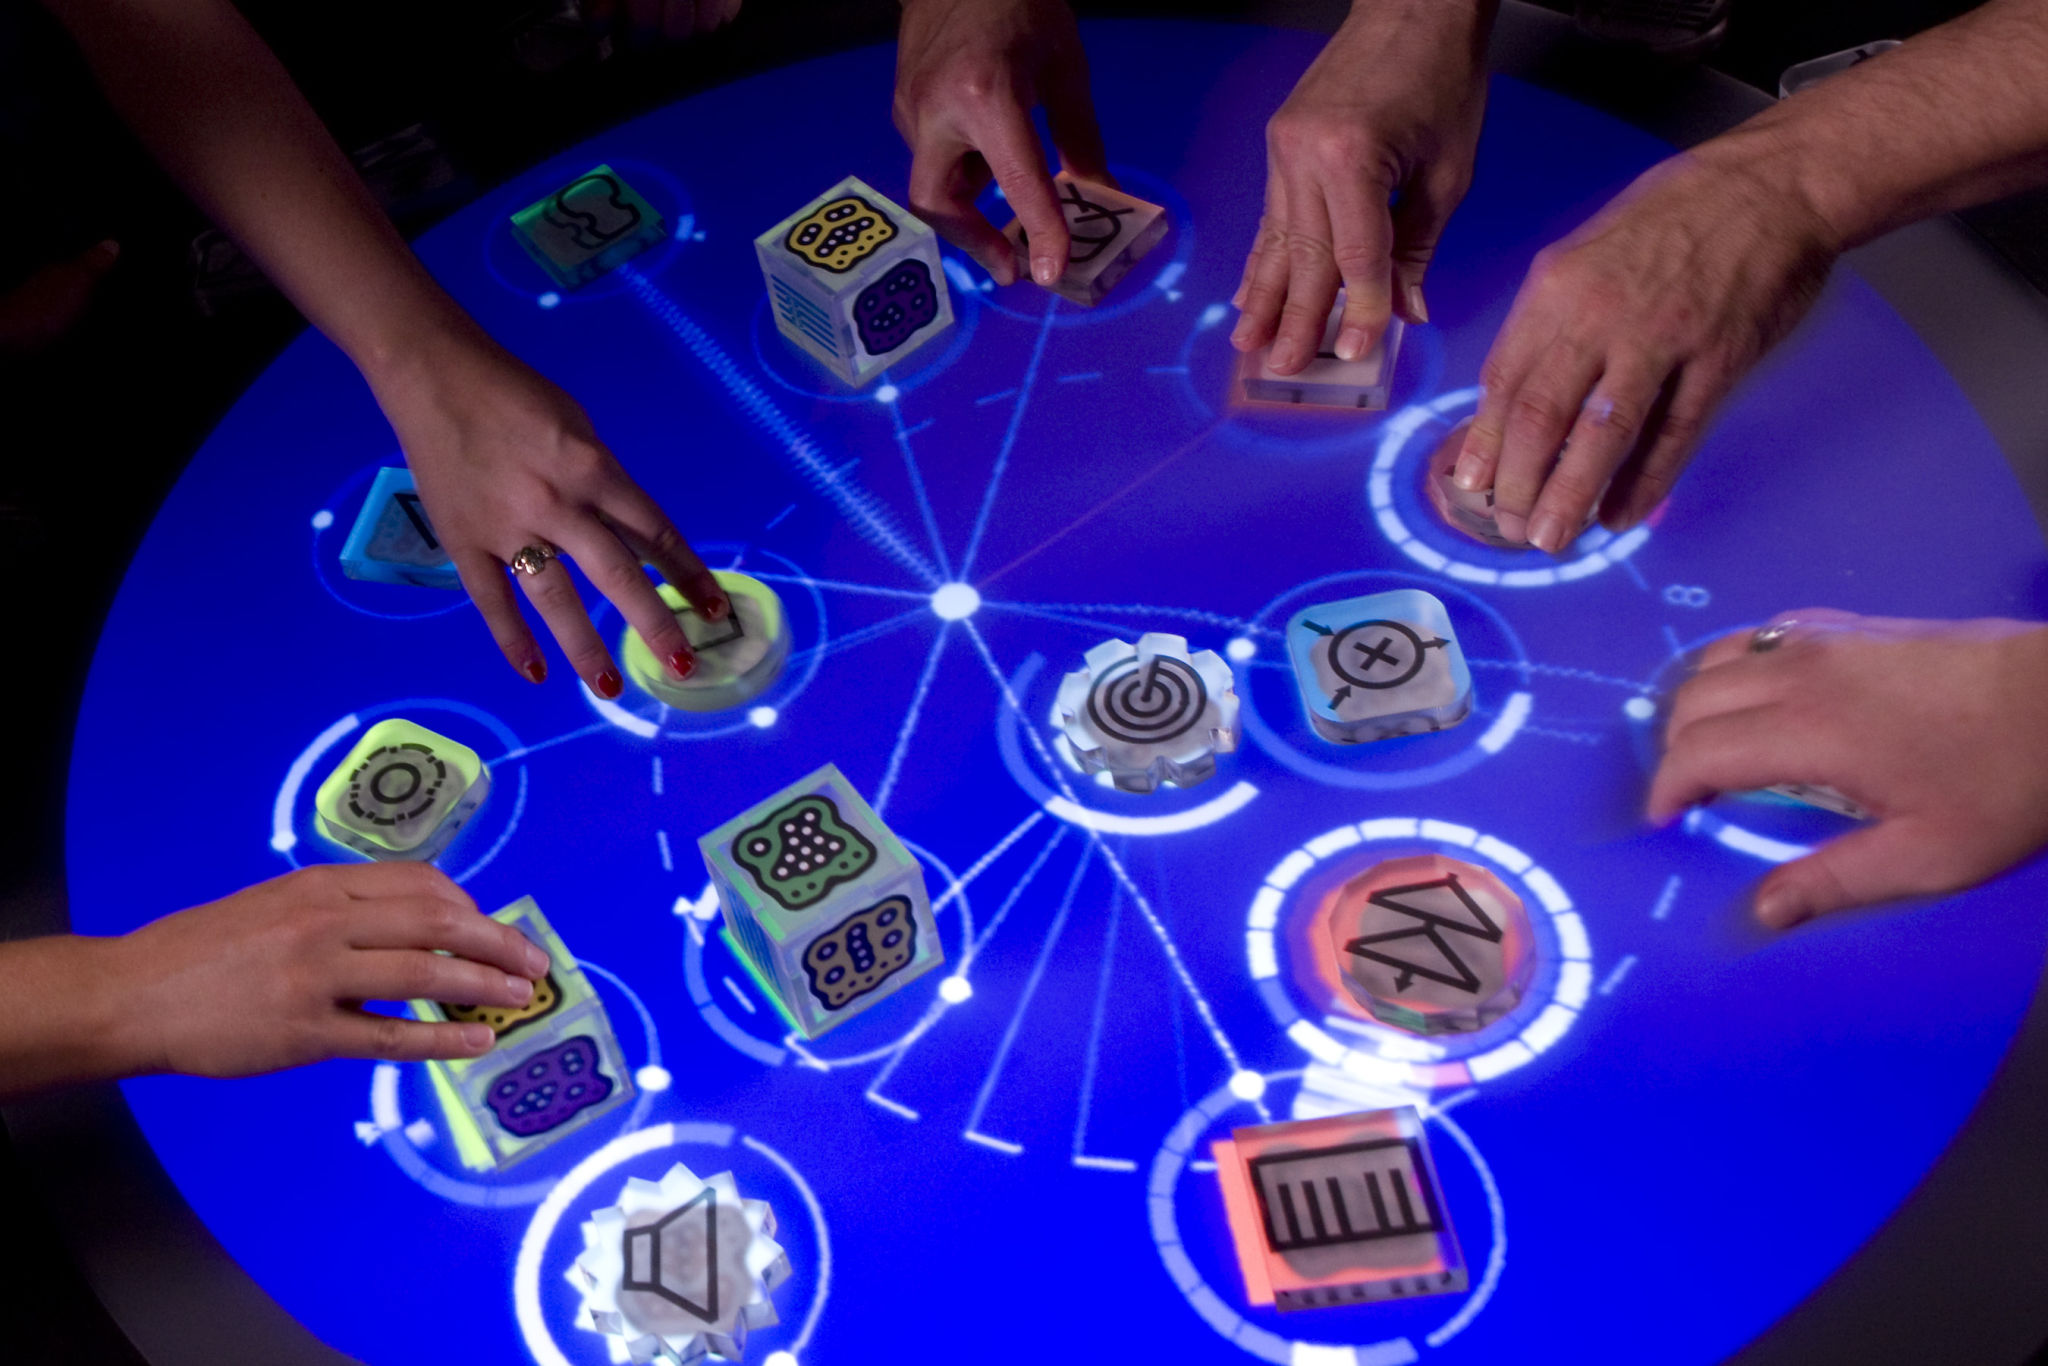
\includegraphics[width=0.6\linewidth]{figure/Analysis/reactable}
					\caption{The Reactable table synthesizer used by multiple users.}
					\label{fig:reactable}
				\end{figure} 
			
		
		\subsection{SketchUp}
			SketchUp\footnote{SketchUp: \url{https://www.sketchup.com/}} is a 3D modeling tool that allows for a user to create 2D lines and shapes, which can be manipulated through vertex editing turning it into 3D models in a simplistic fashion. When the 3D models are created SketchUp offers different functionalities for bringing details to the product, and then creating layout drawings from the final	model e.g. to show customers a house drawing or even landscape architecture. The software has it strengths and weaknesses in its simplicity, since it allows for intuitive modelling, but falls off on immersion making the designs seem stale. All though that could be seen as a weakness, it enables minimal memory usage to allow for a highly effortless experience. \\
			
			SkethUp exists in various versions for different professions like architecture, construction, engineering, landscape architecture and the like. Creators are enabled to share their models with the community, or save them for their own later use, to implement in bigger structure planning eg. a tree could be saved as an asset to use for a complete garden design.
				\begin{figure}[H]
					\centering
					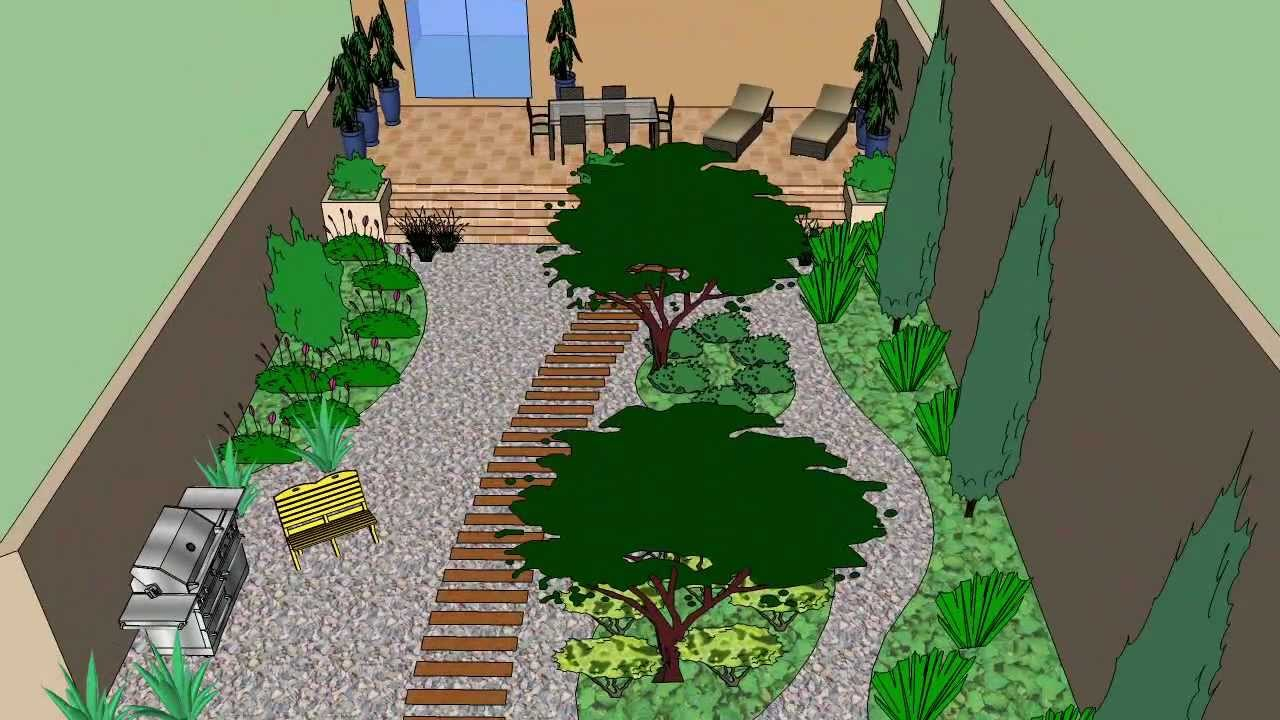
\includegraphics[width=0.6\linewidth]{figure/Analysis/sketchupgarden}
					\caption{A garden designed in SketchUp}
					\label{fig:sketchupgarden}
				\end{figure}